\vspace*{1em}

{\bf Ideas of Partnership.}
\begin{example}[additive]
Compute $1 + 2+ 3 + \cdots + 49$.
\[\begin{tikzcd}[column sep=0.01pt]
\fbox{$1$} \arrow[rrrrrrrrdddddddd, "{\textnormal{sum}\, =\, 50}" description, bend right,no head] & + & \fbox{$2$} \arrow[rrrrrrdddddd, "{\textnormal{sum}\, =\, 50}" description, bend right,no head] & + & \cdots & + & \fbox{$24$} \arrow[rrdd, "{\textnormal{sum}\, =\, 50}" description, bend right,no head] & + & \fbox{$25$} \\[-0.2in]
                                                                                         &   &                                                                                        &   &        &   &                                                                                 &   & +           \\[-0.2in]
                                                                                         &   &                                                                                        &   &        &   &                                                                                 &   & \fbox{$26$} \\[-0.2in]
                                                                                         &   &                                                                                        &   &        &   &                                                                                 &   & +           \\[-0.2in]
                                                                                         &   &                                                                                        &   &        &   &                                                                                 &   & \vdots      \\[-0.2in]
                                                                                         &   &                                                                                        &   &        &   &                                                                                 &   & +           \\[-0.2in]
                                                                                         &   &                                                                                        &   &        &   &                                                                                 &   & \fbox{$48$} \\[-0.2in]
                                                                                         &   &                                                                                        &   &        &   &                                                                                 &   & +           \\[-0.2in]
                                                                                         &   &                                                                                        &   &        &   &                                                                                 &   & \fbox{$49$}
\end{tikzcd}\]
Therefore, 
\[\textnormal{Sum}= 50\cdot(\card\,\text{pairs}) + 25 = 50\cdot 24 + 25 = 1200 + 25 = 1225\]
\end{example}

\vspace*{1.5em}

\begin{theorem}[Wilson]\label{wilsonthm}
Let $p$ be a prime number. Then we have
\[(p-1)! \equiv -1\modar{p}\]
\end{theorem}
\begin{proof}
Consider $\Phi(p) = \set{1,\,2,\,\ldots,\,p-1}$,
\begin{itemize}[leftmargin=*]
\item[] \emph{Partner} $x \in \Phi(p)$ with $y \in \Phi(p)$ if and only if $xy \equiv 1\modar{p}$. That is, partner $x$ with its multiplicative inverse $y$ modulo $p$.
\item[] \emph{Know:} any $x \in \Phi(p)$ has a unique multiplicative modulo $p$ in $\Phi(p)$.
\item[] \emph{Question.} When is $x \in \Phi(p)$ its own partner?
\item[] \emph{Answer.} It is
\begin{align*}
\iff x\cdot x \equiv 1 \modar{p} \iff& x^2 - 1 \equiv 0 \modar{p}\\[0.5em]
\iff& x^2 - \overline{1} = \overline{0},\text{ in }\ff_p\\[0.5em]
\iff& (x - \overline{1})(x + \overline{1}) = \overline{0}, \text{ in }\ff_p\\[0.5em]
\iff& x = - \overline{1}\ \text{ or }\ x = \overline{1}, \text{ in }\ff_p\\[0.5em]
\iff& x \equiv -1 \equiv p-1\modar{p}\ \text{ or }\ x \equiv 1 \modar{p}
\end{align*}
\end{itemize}
\begin{itemize}[leftmargin=4.5em]
\item[$(p = 2)$] A special case 
\[(p-1)! = (2-1)! = 1! = 1 \equiv -1\modar{2}\]
\item[$(p\geq 3)$] $\Phi(p)$ contains two distinct elements, namely $1$ and $p-1$, that don't get partnered with different elements. All the other elements $x$ get partnered with some $y \neq x$. Therefore
\begin{align*}
(p-1)! &= \text{the product of all elements in $\Phi(p)$.}\\[0.5em]
&= 1\cdot(p-1)\cdot(\text{partnered products})\\[0.5em]
&\equiv (p-1)\cdot 1\modar{p}\\[0.5em]
&\equiv -1\modar{p}\\[-3em]
\end{align*}
\end{itemize}
\end{proof}

\vspace*{1em}

\emph{e.g.} Let $p = 11$, the partnership specified in the proof above is
\[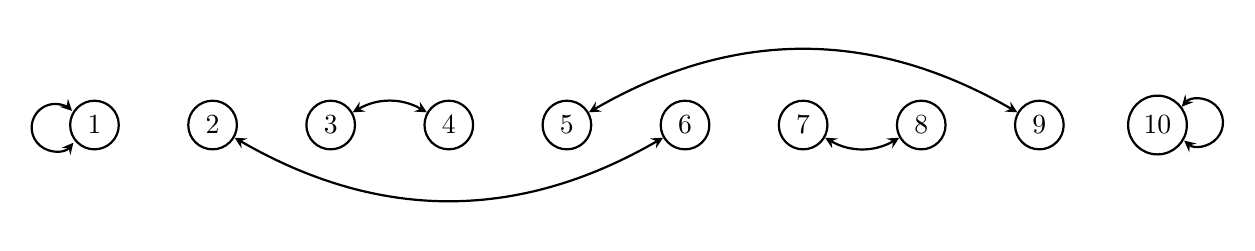
\begin{tikzpicture}[<->,>=stealth,auto,node distance=1.5cm,
  thick,main node/.style={circle,draw}]

  \node[main node] (1) {$1$};
  \draw[]	([shift=(40:-0.35cm)]1) arc (140:-135:-3mm) node[] {} (1);

  \node[main node] (2) [right of=1] {$2$};
  \node[main node] (3) [right of=2] {$3$};
  \node[main node] (4) [right of=3] {$4$};
  \node[main node] (5) [right of=4] {$5$};
  \node[main node] (6) [right of=5] {$6$};
  \node[main node] (7) [right of=6] {$7$};
  \node[main node] (8) [right of=7] {$8$};
  \node[main node] (9) [right of=8] {$9$};
  \node[main node] (10) [right of=9] {$10$};
\draw[]	(10.37) arc (138:-130:3mm) node[] {} (10);
  \path[every node/.style={font=\sffamily\small}]
    (2) edge[bend right] node[] {} (6)
    (5) edge[bend left] node[] {} (9)
    (3) edge[bend left] node[] {} (4)
    (7) edge[bend right] node[] {} (8);
\end{tikzpicture}\]

\vspace*{1.5em}

\begin{proposition}
Let $p$ be an odd prime, so $\card\Phi(p) = p-1$ is even. Then, exactly half $(=(p-1)/2)$ of $\Phi(p)$ are quadratic residues, the other half quadratic non-residues.
\end{proposition}
\begin{proof}
If $x \in \Phi(p)$, then $p\nmid x^2$, so we have a function
\[\Phi(p) \overset{f}{\longrightarrow} \Phi(p),\ x \mapsto x^2\modar{p}\]
Note that $x^2\modar{p}$ here refers to the natural representative of $x^2$ modulo $p$ in $\Phi(p)$.\\
\\
Let $R$ be the image of $f$. By definition, $R$ is the set of quadratic residues in $\Phi(p)$.\\
\begin{subproof}
\vspace*{-0.1in}
{\bf Claim.} The function $\Phi(p) \overset{f}{\longrightarrow} R$ is a two-to-one function. That is, for any $a \in R$, there exist exactly two $x_1,x_2 \in \Phi(p)$ such that $f(x_1) = a = f(x_2)$. Equivalently, $\card{f^{-1}(a)} = 2$.
\begin{proof}[Proof of Claim]
Consider the polynomial $r(T) = T^2 - \overline{a}$, for any $a \in R$, and let $y \in f^{-1}(a)$. Then $a = f(y)$, i.e. $y^2 \equiv a\modar{p}$, or equivalently $r(\overline{y}) = 0$. Therefore, $f^{-1}(a)$ consists of roots of $r(T)$.\\[0.5em]
By definition of $R$, there's atleast one $x_1 \in \Phi(p)$ such that $a = f(x_1)$, i.e. $x_1^2 \equiv a \modar{p}$, or equivalently $r(\overline{x}_1) = 0$. Now, $x_2 = p-x_1 \in \Phi(p)$ also has this property,
\begin{align*}
x_2^2 &= (p-x_1)^2\\[0.5em]
&\equiv (-x_1)^2 \modar{p}\\[0.5em]
&\equiv x_1^2\modar{p}\\[0.5em]
&\equiv a\modar{p}
\end{align*}
Since $\deg r = 2$, these two are necessarily its only roots. Furthermore, note that $x_1 \neq x_2$ as one is odd and the other even, since $x_1 + x_2 = p$, an odd prime. Hence, $\card{f^{-1}(a)} = 2$, as needed. 
\end{proof}
\vspace*{0.05ex}
\end{subproof}
\vspace*{1em}
Since $\card\Phi(p) = p-1$ and $f$ is two-to-one onto $R$. We have, $\card{R} = \dfrac{\card{\Phi(p)}}{2} = \dfrac{p-1}{2}$.
\end{proof}

\vspace*{1.5em}

\begin{definition}
Let $p$ be a prime number and $a,\,x,\,y \in \Phi(p)$. Say that $x$ and $y$ are $a$-partners if
\[xy \equiv a \modar{p}\]
\end{definition}
\emph{e.g.} Let $p = 11$,
\begin{itemize}[leftmargin=*,itemsep=2em]
\item[] $a=1$, this $1$-partnership is what we used in the proof of Theorem \ref{wilsonthm}.
\item[] $a = 2$,
\[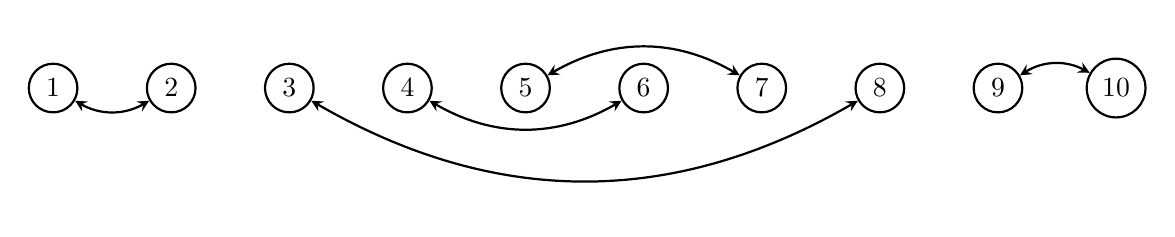
\begin{tikzpicture}[<->,>=stealth,auto,node distance=1.5cm,
  thick,main node/.style={circle,draw}]

  \node[main node] (1) {$1$};
  \node[main node] (2) [right of=1] {$2$};
  \node[main node] (3) [right of=2] {$3$};
  \node[main node] (4) [right of=3] {$4$};
  \node[main node] (5) [right of=4] {$5$};
  \node[main node] (6) [right of=5] {$6$};
  \node[main node] (7) [right of=6] {$7$};
  \node[main node] (8) [right of=7] {$8$};
  \node[main node] (9) [right of=8] {$9$};
  \node[main node] (10) [right of=9] {$10$};
  \path[every node/.style={font=\sffamily\small}]
    (1) edge[bend right] node[] {} (2)
    (3) edge[bend right] node[] {} (8)
    (5) edge[bend left] node[] {} (7)
    (9) edge[bend left] node[] {} (10)
    (4) edge[bend right] node[] {} (6);
\end{tikzpicture}\]
\item[] $a = 3$,
\[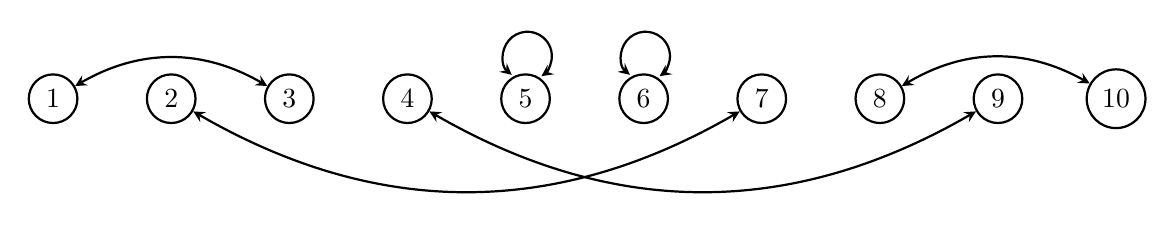
\begin{tikzpicture}[<->,>=stealth,auto,node distance=1.5cm,
  thick,main node/.style={circle,draw}]

  \node[main node] (1) {$1$};
  \node[main node] (2) [right of=1] {$2$};
  \node[main node] (3) [right of=2] {$3$};
  \node[main node] (4) [right of=3] {$4$};
  \node[main node] (5) [right of=4] {$5$};
\draw[]	([shift=(120:0.35cm)]5) arc (230:-55:3.1mm) node[] {} (5);
  \node[main node] (6) [right of=5] {$6$};
  \node[main node] (7) [right of=6] {$7$};
  \node[main node] (8) [right of=7] {$8$};
  \node[main node] (9) [right of=8] {$9$};
  \node[main node] (10) [right of=9] {$10$};
\draw[]	([shift=(120:0.35cm)]6) arc (230:-55:3.1mm) node[] {} (6);
  \path[every node/.style={font=\sffamily\small}]
    (1) edge[bend left] node[] {} (3)
    (4) edge[bend right] node[] {} (9)
    (8) edge[bend left] node[] {} (10)
    (2) edge[bend right] node[] {} (7);
\end{tikzpicture}\]
\end{itemize}

\vspace*{0.5em}

\begin{remark}
We note that every $x \in \Phi(p)$ has an $a$-partner. This is because any such $x$ has a multiplicative inverse $z$ modulo $p$, that is $xz \equiv 1 \modar{p}$. Then taking $y \in \Phi(p)$ to be such that $y \equiv az \modar{p}$ (that is, $y$ is the natural representative of $az$ modulo $p$) we have 
\[xy \equiv a(xz) \equiv a \modar{p}\]
Hence $y$ is an $a$-partner of $x$.
\end{remark}

\vspace*{1.5em}

\begin{theorem}[Euler]\label{eulerqr}
Let $p$ be an odd prime, and let $a \in \Phi(p)$. Then
\begin{itemize}
\item[(1)] $a$ is a quadratic residue if and only if $a^{\frac{p-1}{2}} \equiv 1 \modar{p}$.
\item[(2)] $a$ is a quadratic non-residue if and only if $a^{\frac{p-1}{2}} \equiv -1 \modar{p}$.
\end{itemize}
\end{theorem}
\begin{proof}
We first note that by Theorem \ref{fermatlittle} we have
\[a^{p-1} \equiv 1\modar{p}\]
Since $p$ is an odd prime, $p-1$ is even, so we get
\[(a^{\frac{p-1}{2}}-1)(a^{\frac{p-1}{2}}+1) = a^{p-1} - 1 \equiv 0\modar{p}\]
if and only if
\[a^{\frac{p-1}{2}} \equiv 1 \modar{p}\quad \text{or}\quad a^{\frac{p-1}{2}} \equiv -1 \modar{p}.\] From this, we note that the statements in the theorem are contrapositives of each other. Thus, it suffices to prove one of them; we prove (2).\\
\\
($\Leftarrow$) If $a$ is a QNR, then there's \emph{no} $x \in \Phi(p)$ that is its own $a$-partner, because otherwise we have $x^2 = x\cdot x \equiv a \modar{p}$ making $a$ a QR. Recall that every $x \in \Phi(p)$ has an $a$-partner $y \in \Phi(p)$, necessarily with $y \neq x$. Hence, by Corollary \ref{wilsonthm}, we have
\begin{align*}
-1 &\equiv (p-1)!\modar{p}\\[0.5em]
&\equiv (\text{product of elements in $\Phi(p)$})\modar{p}\\[0.5em]
&\equiv a^{\frac{p-1}{2}}\modar{p}
\end{align*}
($\Rightarrow$) Suppose $a^{\frac{p-1}{2}} \equiv -1\modar{p}$ and for the sake of contradiction assume that $a$ is a QR, then there exists an $x \in \Phi(p)$ such that $x^2 \equiv a\modar{p}$. Then
\begin{align*}
x^{p-1} &= (x^2)^{\frac{p-1}{2}}\\[0.5em]
&\equiv a^{\frac{p-1}{2}} \modar{p}\\[0.5em]
&\equiv -1 \modar{p}
\end{align*}
contradicting Corollary \ref{fermatlittle}. Thus, necessarily, $a$ is a QNR.
\end{proof}

\vspace*{1em}

\begin{remark}
Note that if $a \in \Phi(p)$ is a primitive root modulo $p$, then it's necessarily a quadratic non-residue. Since, by definition, $p-1$ is the smallest positive integer such that $a^{p-1} \equiv 1 \modar{p}$. Therefore, necessarily, $a^{\frac{p-1}{2}} \not\equiv 1 \modar{p}$. Hence, $a$ is a QNR.
\end{remark}

\vspace*{1.5em}

\begin{example} 
Determine whether $a = 3$ is a quadratic residue modulo $p = 43$.
\end{example}
\begin{proof}[Answer]
We want to compute $3^{\frac{43-1}{2}}\modar{43} = 3^{21}\modar{43}$. Note,
\allowdisplaybreaks
\begin{align*}
3^1 &\equiv 3 \modar{43}\\[0.5em]
3^2 &\equiv 9 \modar{43}\\[0.5em]
3^4 &\equiv 81 \equiv -5 \modar{43}\\[0.5em]
3^{16} &\equiv (-5)^4 \equiv 125\cdot 5 \equiv(-4)\cdot 5 \equiv-20 \modar{43}
\end{align*}
Therefore,
\begin{align*}
3^{21} = 3^{16+4+1} &\equiv (-20)\cdot (-5)\cdot 3\modar{43}\\[0.5em]
&\equiv 100\cdot 3\modar{43}\\[0.5em]
&\equiv 14\cdot 3\modar{43}\\[0.5em]
&\equiv 42\modar{43} \equiv -1\modar{43}
\end{align*}
Hence, $3$ is a QNR modulo $43$.
\end{proof}

\vspace*{1.5em}

\begin{example}[in-class]
Determine whether $a = 2$ is a quadratic residue modulo $p = 29$.
\end{example}

\vspace*{1em}

\begin{corollary}\label{qrl1}
Let $p$ be an odd prime. Then
\[-1\text{ is a quadratic residue$\modar{p}$ if and if $p \equiv 1 \modar{4}$}\]
Equivalently, $T^2 + \overline{1} \in \ff_p[T]$ is reducible if and only if $p \equiv 1 \modar{4}$.
\end{corollary}
\begin{proof}
By Theorem \ref{eulerqr}, $-1$ is a QR$\modar{p}$ if and only if
\[(-1)^{\frac{p-1}{2}} \equiv 1\modar{p}\]
Now, 
\[(-1)^{\frac{p-1}{2}} = \begin{cases}1 & \text{if $\dfrac{p-1}{2}$ is even}\\[1.5em] -1 & \text{if $\dfrac{p-1}{2}$ is odd} \end{cases}\]\\[0.2em]
Note that $\dfrac{p-1}{2}$ is even if and only if $p-1 = 4k$, for some integer $k$, if and only if $p \equiv 1 \modar{4}$.
\end{proof}

\vspace*{0.5in}

\subsection{Problems}
\vspace{0.1in}

\begin{problem}\label{Problem 16.1}
Let $p$ be an odd prime. Recall that a primitive root modulo $p$ is an integer $g$ such that \[g^{p-1} \equiv 1 \modar{p}\] and for no $0 < e < p-1$ do we have $g^e \not\equiv 1 \modar{p}$. The results that we proved in this lecture can be proved via the existence of $g$ (Theorem \ref{gaussprim}).
\begin{itemize}
\item[(a)] Consider $\ff_p^\times = \ff_p \setminus \set{\overline{0}}$ and let $g$ be a primitive root. Prove that 
\[\ff_p^\times = \setp{\overline{g}^e}{0 \leq e < p-1}\]
\item[(b)] Use a primitive root $g$ to demonstrate that $-1$ is a QR modulo $p$ if and only if $p \equiv 1 \modar{4}$.
\item[(c)] Use a primitive root $g$ to prove Theorem \ref{wilsonthm}, by first showing that
\[(p-1)! \equiv g^{1+2+\cdots+(p-2)}\modar{p}\]
\item[(d)] Given a primitive root $g$, and an integer $a$ such that $a \equiv 0 \modar{p}$, prove that $a$ is a QR modulo $p$ if and only if $a \equiv g^e \modar{p}$ for an even number $e$. Use this to prove Theorem \ref{eulerqr}.
\end{itemize} 
\end{problem}